\documentclass[12pt]{article}

\usepackage{cite}				% Used to cite references and figures
\usepackage{amsmath}			% Used for equation reference
\usepackage{amsfonts}			% Used for equation symbols
\usepackage{subcaption}			% Used for subcaption in subfigures
\usepackage{hyperref}
\usepackage{bookmark}
\usepackage{graphicx}
\usepackage{algorithm,algpseudocode}

\usepackage[bottom=1in, top=1in, left=1in, right=1in]{geometry}

\hypersetup{
	colorlinks = true,
	linkcolor = blue,
	filecolor = magenta,
	urlcolor = black,
	citecolor = blue,
	pdftitle = {Feature Detection in VHDL},
	pdfpagemode = UseOutlines,
}


\begin{document}

	\title{ Feature Detection in VHDL }

	\author{	University of North Texas \\
				Department of Electrical Engineering \\
				CSCE 4760.001 \\ \\
				Nicholas Chiapputo \\
	}

	\maketitle

	\section{Introduction}
		Feature detection is the process of parsing a source image and detecting a set of defined features such as edges, corners, blobs, and ridges. These techniques can be combined and refined for specific implementations in order to detect more complex shapes such as faces, animals, and specific patterns. The most common feature detectors are edge detectors. This family of algorithms look for edges in an image by detecting the intensity differences between pixels. 
 
		Generally, image processing can be a processor heavy task and can rely on high-level languages such as C, Python, or Java. While this is good for regular use, it is not very mobile. That is, an embedded system that needs to process images and look for features needs a system to do so without needing to be hooked up to a large machine or require large amounts of data sent over the air. By implementing such feature detections on FPGAs, the world of image processing can be mobile, allowing for rapid, in the field processing without necessitating large devices or requiring an operator. 

		The project seeks to implement the Sobel edge detection algorithm using VHDL in Xilinx's Vivado development environment. Admittedly, Sobel is not the most complex algorithm. However, by implementing Sobel, the baseline is set up for the majority of other algorithms. For example, two of the three steps in Canny edge detection are simply Sobel and the third step is non-maximum suppression to simply find the largest edge. The majority of the difficult work is in setting up the I/O systems to be able to handle large streams of data and be able to appropriately save it for re-use in other components of the system. 

		In \autoref{sec:background}, we cover some information regarding Sobel and Canny edge detection and convolution in image processing. Then \autoref{sec:implementation} describes the implementation of Sobel in VHDL and \autoref{sec:results} details the results of the experiment. The paper is then concluded with \autoref{sec:conclusion}.

	\section{Background}
		\label{sec:background}

		Feature detection covers a wide array of different algorithms that each detect different types of features. Generally, feature detection is the first step in a more complex computer vision algorithm. The algorithm will first look for basic features within an image as input to more detailed and specific operations. Before feature detection, a blur is usually applied to remove excess noise in an image. Blurs are applied using convolutional operators by multiplying a given kernel with a section of the image in element-wise matrix multiplication. 

		\subsection{Convolution}
			Convolution is the sliding multiplication of a kernel $\omega$ with an image region $f(x,y)$ to produce a gradient output $g(x,y)$. This gives the summation of each element of the local neighbors to the target pixel and then weights that sum by the kernel. When calculating the value of the convolution $\omega * f(x,y)$ of a pixel at row $x$ and column $y$ in an image, the summation of the element-wise multiplication of the kernel and image matrices is calculated using the general convolution formula in \eqref{eq:conv}.

			\begin{equation}
				\label{eq:conv}
				g(x, y) = \omega * f(x, y) = \sum_{dx = -a}^{a}{\sum_{dy = -b}^{b}{\omega(dx, dy)f(x + dx, y + dy)}}
			\end{equation}

			A toy example of this is shown with kernel \eqref{eq:exampleKernel} and image region \eqref{eq:exampleImage}. This example kernel value is a simple Gaussian kernel where the values going out from the center pixel are determined from a normal distribution given a standard deviation $\sigma$. The full example is shown in \eqref{eq:exampleKernelCalc} where the gradient $g(2, 2)$ is calculated.

			\begin{equation}
				\omega = 
				\frac{1}{16}
				\begin{pmatrix}
					\label{eq:exampleKernel}
					1 	& 2 	& 1 \\
					2 	& 4 	& 2 \\
					1 	& 2 	& 1 \\
				\end{pmatrix}
			\end{equation}

			\begin{equation}
				f(x,y) =
				\begin{pmatrix}
					\label{eq:exampleImage}
					5 	& 5 	& 5 	& 10 	& 10 \\
					5 	& 5 	& 5 	& 10 	& 10 \\
					5 	& 5 	& 5 	& 10 	& 10 \\
					5 	& 5 	& 5 	& 10 	& 10 \\
					5 	& 5 	& 5 	& 10 	& 10 \\
				\end{pmatrix}
			\end{equation}

			\begin{align}
				g( 2, 2 ) = \omega * f( 2, 2 ) = 	&( 1 \cdot 5 ) + ( 2 \cdot 5 ) + ( 1 \cdot 10 ) + \nonumber\\	
													&( 2 \cdot 5 ) + ( 4 \cdot 5 ) + ( 2 \cdot 10 ) + \\
													&( 1 \cdot 5 ) + ( 2 \cdot 5 ) + ( 1 \cdot 10 )   \nonumber\\
													& = 100 / 16 = 6.25 \nonumber
				\label{eq:exampleKernelCalc}
			\end{align}

			The kernel is generally chosen such that it has an odd number of rows and columns. This allows it to center around the target pixel, instead of being slightly off center. The convolution operator is used both when blurring an image and when calculatig the gradient during Sobel edge detection. While the Sobel kernels generally stay constant, the blurring kernel depends on many factors including which type of blurring is being implemented (e.g., Gaussian or mean) and what parameters are chosen for the specific imlementation as they can significantly effect the performance of the feature detector.

		\subsection{Edge Detection}
			There is no specific definition as to what constitutes a feature of an image. Though it can generally be accepted that any ``interesting'' part of an image can be called a feature. The most specific characteristic of a feature is that it is repeatable. For example, edges are very common in images and repeat in many locations. However, something uncommon like a very specific color pattern or an unusual shape likely won't show up multiple times in an image. 

			With this crude definition, we can focus on the more common feature detection algorithms. Feature detection is generally a low-level image processing operation and is usually one of the first operations done. Because of this, it deals with regular image data (i.e., RGB images). In order to remove unnecessary information from the iamge, we use feature detectors to pick and choose what we take out of the image for further, more complex processing.

			One of the most common types of features is an edge. An edge is simply defined as points where there is a boundary between two regions of differing intensity values. That is, a difference in intensity like the one shown between the second and third columns of \eqref{eq:edgemat}. 

			\begin{equation}
				\begin{pmatrix}
					\label{eq:edgemat}
					50	& 50	& 50	& 100	& 100 \\
					50	& 50	& 50	& 100	& 100 \\
					50	& 50	& 50	& 100	& 100 \\
					50	& 50	& 50	& 100	& 100 \\
					50	& 50	& 50	& 100	& 100 \\
				\end{pmatrix}
			\end{equation}

			Two of the most well-known edge detection algorithms are Canny edge detection, developed by John F. Canny in 1986, and Sobel edge detection developed by Irwin Sobel and Gary Feldmen in 1968. These are classic algorithms that are still in use today, albeit for mainly academic purposes as there are more complex and more specific detectors now. The steps of Canny edge detection completely envelop the steps of Sobel. That is, Sobel is part of Canny, which then takes a few extra steps afterwards. We will first discuss Sobel and then briefly explain the extra steps Canny takes.

			Sobel edge detection takes part in three different phases. First, the source image is converted to a grayscale image. This servers two purposes - first it has the ability to further sharpen contrast in an image and second it can reduce the complexity of operations as we no longer have to consider color in the image. This is generally not a very important step, but it is common across the majority of feature detection algorithms, so it is important to note when describing how an algorithm works. An example grayscaling of an image is shown in \autoref{fig:grayscale}. This images shows that some features, such as the fur on the face, can be somewhat enhanced with grayscaling while others, such as the grass, lose some sharpness.

			\begin{figure}[H]
				\centering
				\begin{subfigure}[b]{0.45\linewidth}
					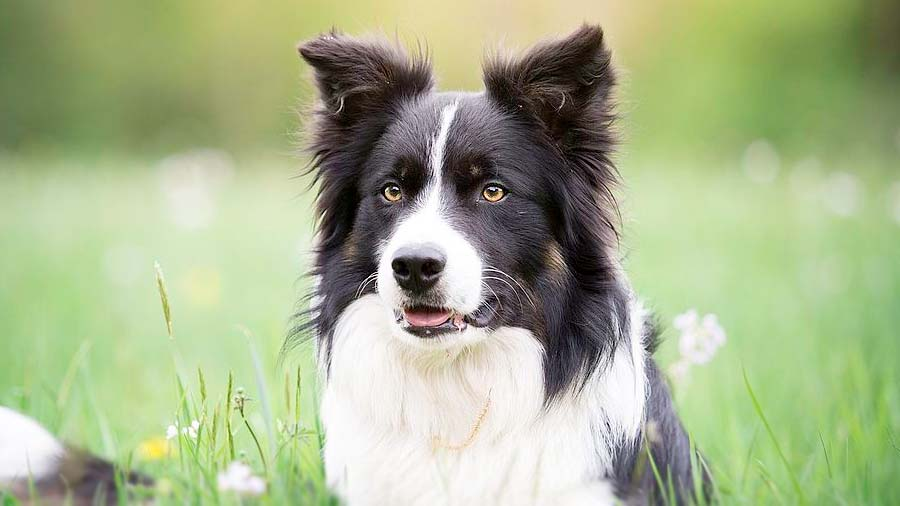
\includegraphics[width=1\linewidth,keepaspectratio]{../examples/dog/bc}
					\subcaption{}
					\label{fig:gaussian9x9orig}
				\end{subfigure} %
				\begin{subfigure}[b]{0.45\linewidth}
					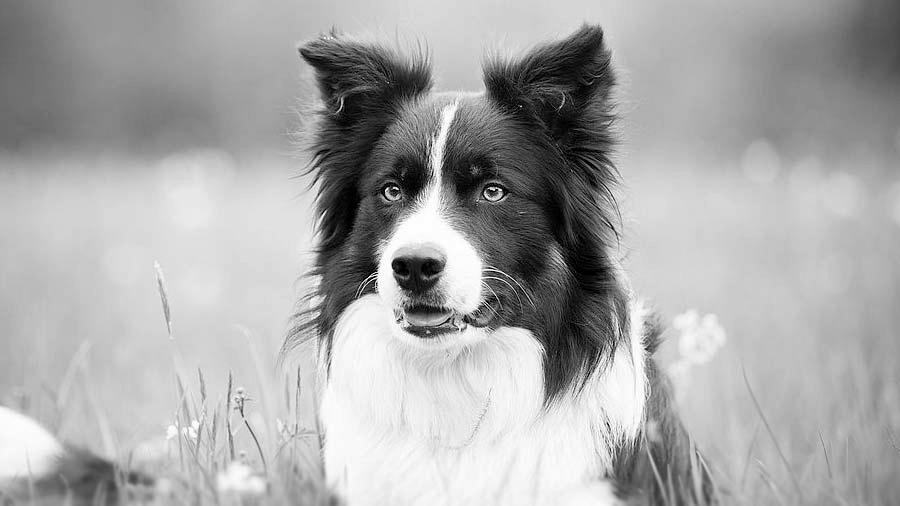
\includegraphics[width=1\linewidth,keepaspectratio]{../examples/dog/dog_gray}
					\subcaption{}
					\label{fig:gaussian9x9blur}
				\end{subfigure} %
				\caption{\small (a) Original image and (b) grayscaled image.}
				\label{fig:grayscale}
			\end{figure} %

			The second step of the Sobel algorithm is blurring. When blurring an image, small noise is removed while preserving the stronger edges. When images are taken with a digital camera, there will inevitably be some noise in the image. By blurring the image, these samll noise values are averaged out. This prevents the algorithm from incorrectly marking those locations as edges. Blurring is done by convolving a kernel over the grayscaled image.

			Gaussian blurring is the most widely used form of blurring. The kernel values for Gaussian blurring are based on a normal distribution. Indexes further away from the center of the kernel are weighted based on a standard devation $\sigma$ of a normal distribution. An example 9x9 Gaussian kernel generated with a $\sigma$ of 3 is shown in \eqref{eq:gaussian9x9}. 

				\begin{equation}
					\frac{1}{999}
					\begin{pmatrix}
						\label{eq:gaussian9x9}
						4 	& 6 	& 8		& 9 	& 10 	& 9 	& 8 	& 6 	& 4 \\
						6 	& 9 	& 11	& 13	& 14 	& 13 	& 11 	& 9 	& 6 \\
						8 	& 11 	& 15	& 18 	& 19 	& 18 	& 15 	& 11 	& 8 \\
						9 	& 13 	& 18	& 21 	& 22 	& 21 	& 18 	& 13 	& 9 \\
						10 	& 14 	& 19	& 22 	& 23 	& 22 	& 19 	& 14 	& 10 \\
						9 	& 13 	& 18	& 21 	& 22 	& 21 	& 18 	& 13 	& 9 \\
						8 	& 11 	& 15	& 18 	& 19 	& 18 	& 15 	& 11 	& 8 \\
						6 	& 9 	& 11	& 13	& 14 	& 13 	& 11 	& 9 	& 6 \\
						4 	& 6 	& 8		& 9 	& 10 	& 9 	& 8 	& 6 	& 4 \\
					\end{pmatrix}
				\end{equation}

			\begin{figure}[H]
				\centering
				\begin{subfigure}[b]{0.45\linewidth}
					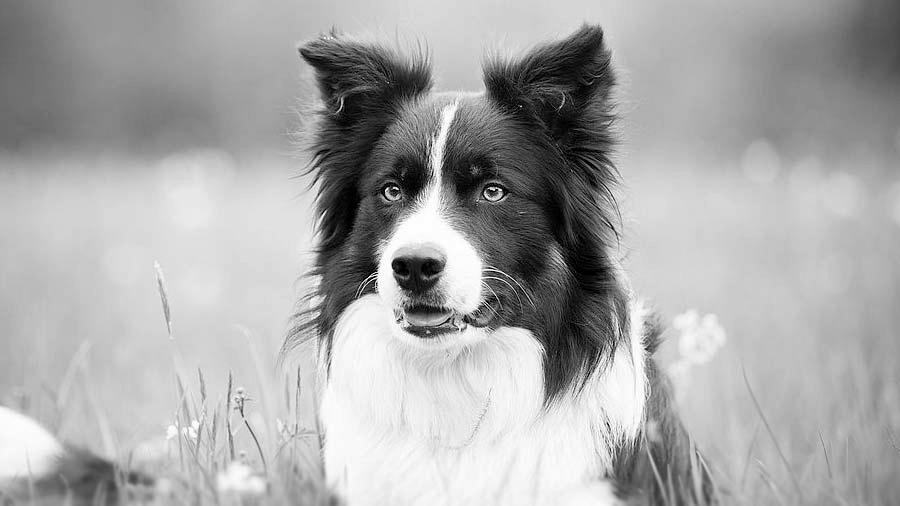
\includegraphics[width=1\linewidth,keepaspectratio]{../examples/dog/dog_gray}
					\subcaption{}
					\label{fig:gaussian9x9orig}
				\end{subfigure} %
				\begin{subfigure}[b]{0.45\linewidth}
					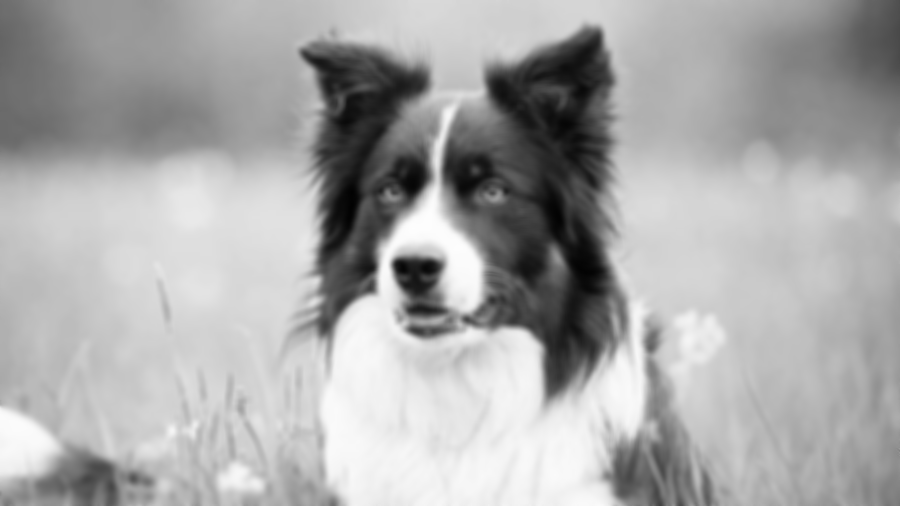
\includegraphics[width=1\linewidth,keepaspectratio]{../examples/dog/dog_gaussian-9x9}
					\subcaption{}
					\label{fig:gaussian9x9blur}
				\end{subfigure} %
				\caption{\small (a) Grayscaled image and (b) blurred image using 9x9 Gaussian kernel with $\sigma$ of 3.}
				\label{fig:gaussian9x9}
			\end{figure} %

			This specific kernel was used in many of the tests for this implementation and has shown good results. It blurs the image sufficiently well to get rid of small details while still preserving strong edges and larger details. An example of the blurring is shown in \autoref{fig:gaussian9x9}.

			Once the image is blurred, the actual edge detection can take place. In Sobel, this is a very simple calculation. To determine the intensity of the edge values, gradients at each pixel are calculated by applying the Sobel-operator. The Sobel-operator is the x- and y-direction gradients $K_{GX}$ and $K_{GY}$ as defined in \eqref{eq:sobelx} and \eqref{sobely}. 

			\begin{equation}
				K_{GX} = 
				\begin{pmatrix}
					\label{eq:sobelx}
					-1	& 0	& 1 \\
					-2	& 0	& 2 \\
					-1	& 0 & 1 \\
				\end{pmatrix}
			\end{equation}

			\begin{equation}
				K_{GY} = 
				\begin{pmatrix}
					\label{eq:sobely}
					1	& 2		& 1 \\
					0	& 0		& 0 \\
					-1	& -2 	& -1 \\
				\end{pmatrix}
			\end{equation}

			The resulting gradients of each the convolutions, $K_{GX}$ (vertical gradient) and $K_{GY}$ (horizontal gradient) are squared and summed and then the square root is taken of that value to get the magnitude of the gradient. 

			The result of the convolution using the kernels produces the x- and y-direction gradients $G_x$ and $G_y$. The magnitude of these results is then determined using $\sqrt{G_{x}^{2} + G_{y}^{2}}$. This gradient magnitude values is then compared to a threshold value that is a parameter of the Sobel algorithm. If the magnitude is greater than the threshold, it is added to the image. Otherwise, the value is replaced with a black pixel to denote no edges. This threshold value is useful for getting rid of small edges or excess noide in an image.

			The Canny algorithm uses the Sobel algorithm as a springboard and adds a few extra steps. First, it takes the gradient magnitudes from Sobel and calculates the angle of the edge $\Theta = \text{tan}^{-1}\left(\frac{G_y}{G_x}\right)$. The algorithm then uses non-maximum suppression in order to thin the edges by effectively combining multiple nearby small edges to form one singular edge. This is done by suppressing all the gradient values except the local maxima, adjusting the blurred edges from Sobel detection to sharper, cleaner edges.

			The Canny algorithm then utilizes double thresholding. Whereas Sobel only uses one threshold value, Canny uses both an upper and a lower threshold value. As with Sobel, if the gradient magnitude is greater than the high threshold, it is added to the image. The difference in Canny is that, if the gradient is in between the high and low threshold values, the edge is marked as weak and is added as a muted gray value to the output image. If the magnitude is lower than the low threshold, then the edge is not added to the image, as in Sobel.

			\begin{figure}[H]
				\centering
				\begin{subfigure}[b]{0.45\linewidth}
					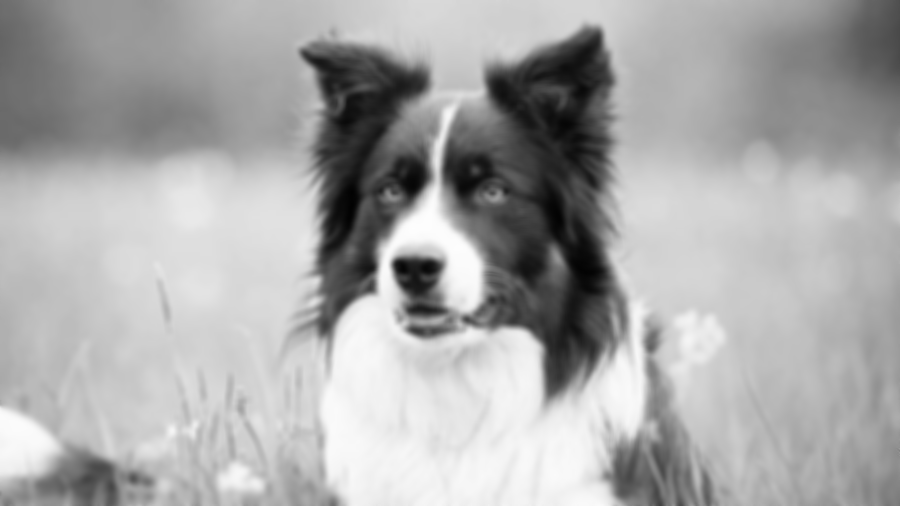
\includegraphics[width=1\linewidth,keepaspectratio]{../examples/dog/dog_gaussian-9x9}
					\subcaption{}
					\label{fig:sobel_blur}
				\end{subfigure} %
				\begin{subfigure}[b]{0.45\linewidth}
					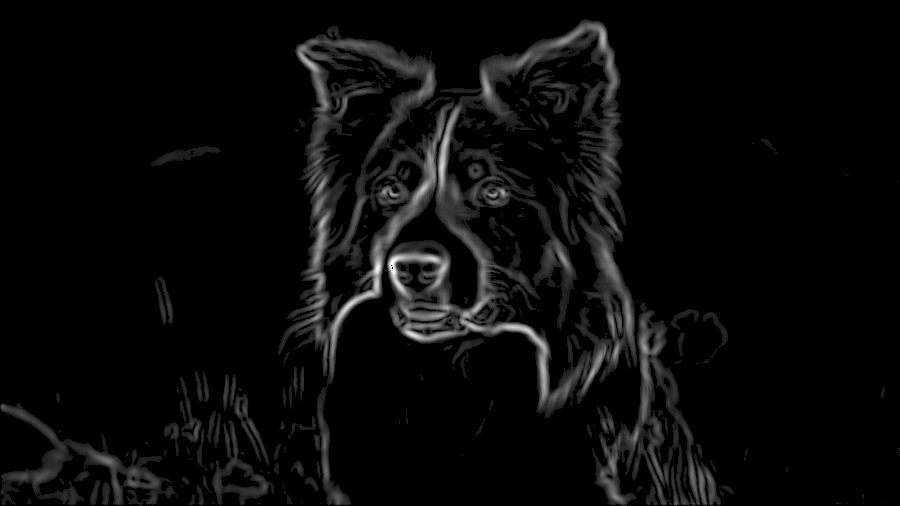
\includegraphics[width=1\linewidth,keepaspectratio]{../examples/dog/dog_gaussian-9x9_thresh-25}
					\subcaption{}
					\label{fig:sobel_out}
				\end{subfigure} %
				\caption{\small (a) blurred image using 9x9 Gaussian kernel with $\sigma$ of 3 and (b) Sobel output image using a threshold of 25.}
				\label{fig:sobel}
			\end{figure} %

			At the end of either the Canny or Sobel algorithm, or any other edge detection algorithm, the output image will be a simple black and white image. Black areas denote the absence of edges and higher intensity areas denote edges with the strength of the intensity being directly related to the sharpness of the edge (i.e., a smooth edge will be muted while a sharp edge will be nearly full white). Following the previous example images, the output of the Sobel algorithm is shown in \autoref{fig:sobel} with the previously blurred image. This image used a threshold value of 25.

	\section{Implementation}
		\label{sec:implementation}
		The implementation of the Sobel algorithm is written in VHDL and simulated using Xilinx's Vivado development environment. The top-level design source file is \texttt{edge.vhd}. In this source, there are three components instantiated to execute the Sobel algorithm. The first component is \texttt{file\_input}. This links to the source file \texttt{file\_input.vhd} which opens the image given in the generic port map, reads the RGB byte data, and converts it to grayscale by averaging. The grayscale data is then written to an output file and is saved. The single byte gray data is also saved to a custom typed two-dimensional array.

		This two-dimensional array is then used as input to the second component - the Gaussian blur component which instantiates the soruce file \texttt{gaussian\_blur.vhd}. In this source file, the grayscaled two-dimensional array data is blured using a pre-determined Gaussian kernel. The kernel is set in the test bench and is defined in a custom package \texttt{kernel\_pkg}. This package defines a function that takes in a single integer value and returns the corresponding Gaussian kernel. This is used in the testbench, \texttt{tb\_edge.vhd}, with the input as the constant value \texttt{GAUSSIAN\_KERNEL\_ROWS}. This constant is also defined in \texttt{kernel\_pkg}. In order to change the size of the Gaussian kernel used, the constants \texttt{GAUSSIAN\_KERNEL\_ROWS} and \texttt{GAUSSIAN\_KERNEL\_COLS} must be changed in this package.

		After the blurred image is calculated, it is written out to a separate file. The blurred byte data is also stored into a separate two-dimensional array which is used as input into the third component of the system - the Sobel edge detector. This component links to the source file \texttt{sobel.vhd}. In this file, the gradient values are calculated and the magnitude is determined based off of the blurred image data saved in the Gaussian blur component. The threshold value is determined based off of a generic port map from the testbench. The final data calculated here is saved into an output image file on the system. Once the Sobel operator is complete, the simulation will terminate, as the testbench checks for a boolean output value from the top-level that is connected to the output of the Sobel component. 

	\section{Results}
		\label{sec:results}
		\begin{figure}[H]
			\centering
			\begin{subfigure}[b]{0.45\linewidth}
				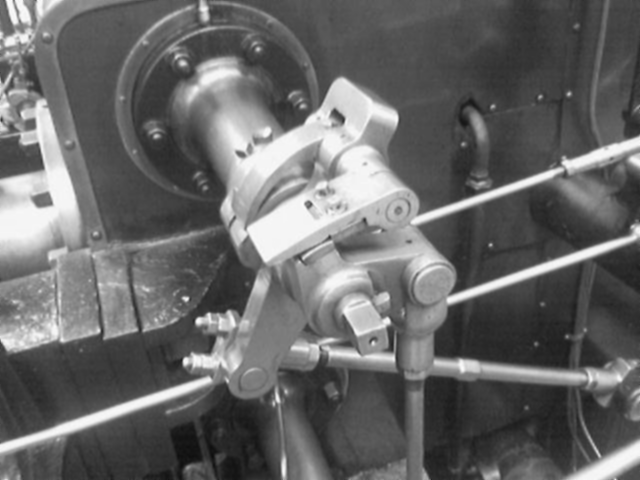
\includegraphics[width=1\linewidth,keepaspectratio]{../examples/valve/valve_gaussian-3x3}
				\subcaption{}
				\label{fig:gaussianCmp3x3}
			\end{subfigure} %
			\begin{subfigure}[b]{0.45\linewidth}
				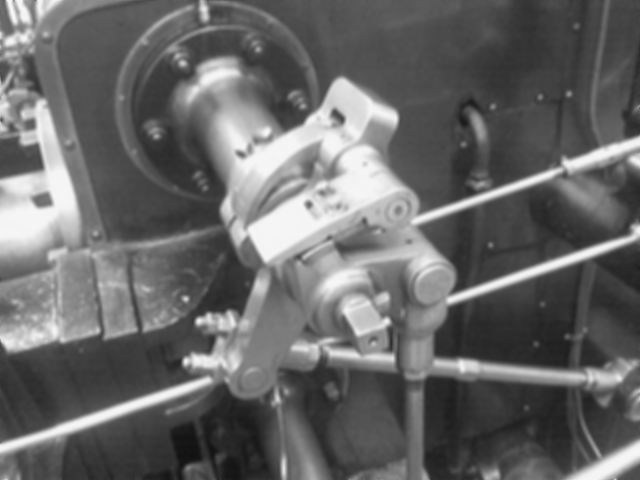
\includegraphics[width=1\linewidth,keepaspectratio]{../examples/valve/valve_gaussian-5x5}
				\subcaption{}
				\label{fig:gaussianCmp5x5}
			\end{subfigure} %
			\begin{subfigure}[b]{0.45\linewidth}
				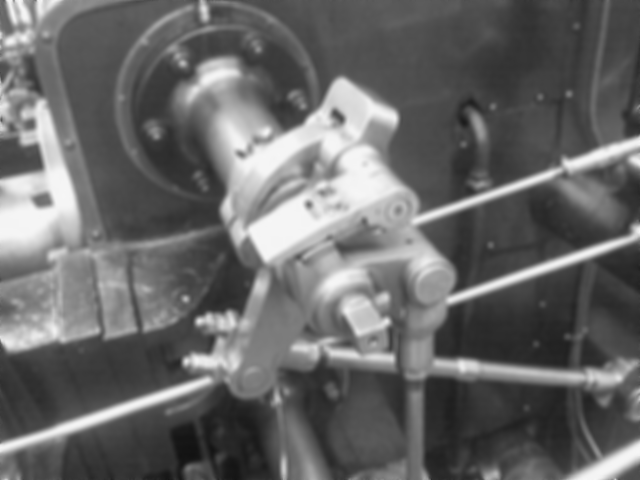
\includegraphics[width=1\linewidth,keepaspectratio]{../examples/valve/valve_gaussian-7x7}
				\subcaption{}
				\label{fig:gaussianCmp7x7}
			\end{subfigure} %
			\begin{subfigure}[b]{0.45\linewidth}
				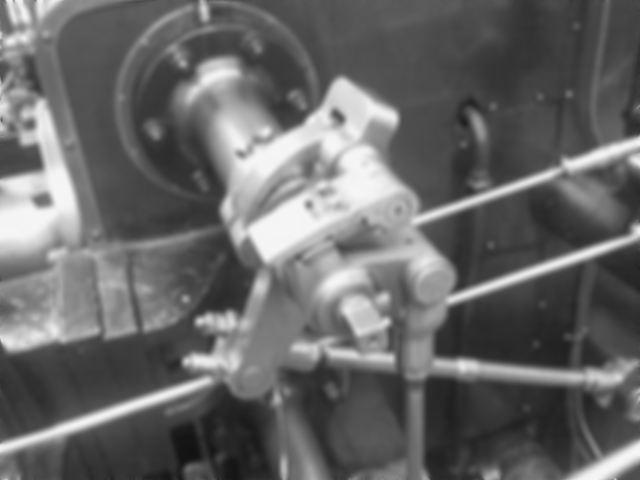
\includegraphics[width=1\linewidth,keepaspectratio]{../examples/valve/valve_gaussian-9x9}
				\subcaption{}
				\label{fig:gaussianCmp9x9}
			\end{subfigure} %
			\caption{\small Comparison of Gaussian kernel sizes using (a) 3x3, (b) 5x5, (c) 7x7, and (d) 9x9. All were generated using $\sigma = 3$.}
			\label{fig:gaussianCmp}
		\end{figure} %

		To test the effectiveness of the implementation, multiple images were used as input. From here, four different Gaussian kernels were tested - 3x3, 5x5, 7x7, and 9x9 - all with $\sigma = 3$. To verify that the Gaussian blurring works as intended, they can be compared side-by-side as in \autoref{fig:gaussianCmp}. From this figure, we can see that the higher kernel sizes lead to a more blurred image. This makes sense given that a larger kernel means that more pixels are taking place in the averaging for each individual pixel. Thus, from this figure, we can conclude that the Gaussian blurring implementation works as expected.

		\begin{figure}[H]
			\centering
			\begin{subfigure}[b]{0.45\linewidth}
				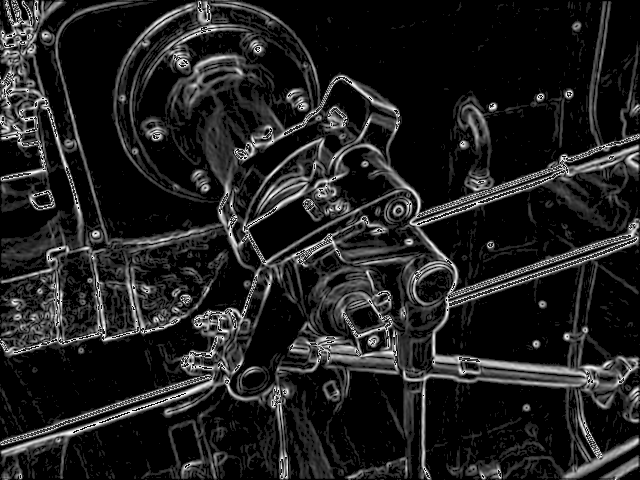
\includegraphics[width=1\linewidth,keepaspectratio]{../examples/valve/valve_gaussian-3x3_thresh-25}
				\subcaption{}
				\label{fig:sobelGaussianCmp3x3}
			\end{subfigure} %
			\begin{subfigure}[b]{0.45\linewidth}
				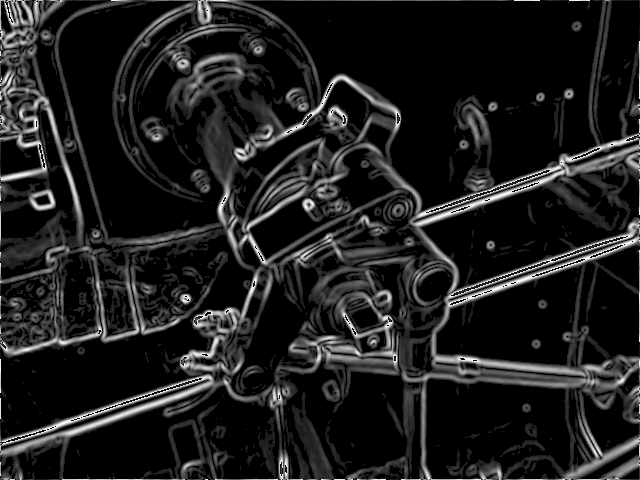
\includegraphics[width=1\linewidth,keepaspectratio]{../examples/valve/valve_gaussian-5x5_thresh-25}
				\subcaption{}
				\label{fig:sobelGaussianCmp5x5}
			\end{subfigure} %
			\begin{subfigure}[b]{0.45\linewidth}
				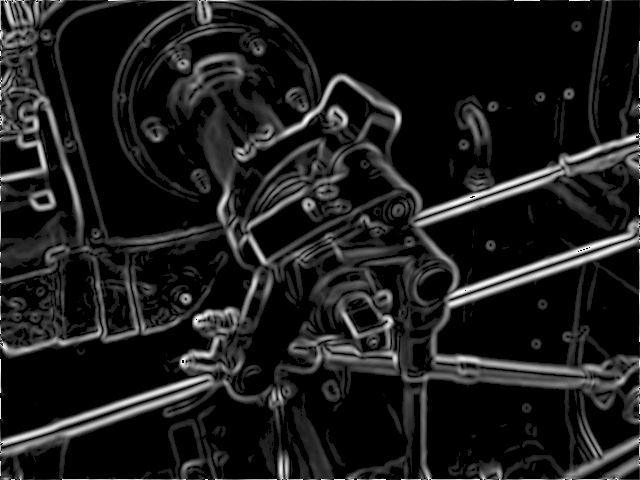
\includegraphics[width=1\linewidth,keepaspectratio]{../examples/valve/valve_gaussian-7x7_thresh-25}
				\subcaption{}
				\label{fig:sobelGaussianCmp7x7}
			\end{subfigure} %
			\begin{subfigure}[b]{0.45\linewidth}
				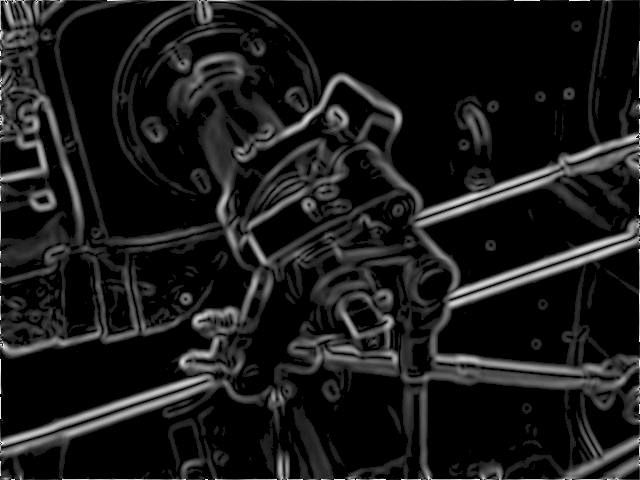
\includegraphics[width=1\linewidth,keepaspectratio]{../examples/valve/valve_gaussian-9x9_thresh-25}
				\subcaption{}
				\label{fig:sobelGaussianCmp9x9}
			\end{subfigure} %
			\caption{\small Comparison of Sobel output for Gaussian kernel sizes of (a) 3x3, (b) 5x5, (c) 7x7, and (d) 9x9. All were generated using $\sigma = 3$.}
			\label{fig:sobelGaussianCmp}
		\end{figure} %

		Similarly for the Sobel edge detection, we can compare both different Gaussian kernel sizes as well as different threshold values. In \autoref{fig:sobelGaussianCmp}, the same four figures from \autoref{fig:gaussianCmp} are fed into the Sobel implementation. For these images, a threshold of 25 is kept constant so that the only variable effecting the different outcomes is the Gaussian kernel size. From these images, we can see that an increase in kernel size removes some of the finer details, leaving the larger edges to be more prominent. This is directly as expected, since blurring an image removes noise and fine details while still preserving the harsher edges. 

		\begin{figure}[H]
			\centering
			\begin{subfigure}[b]{0.45\linewidth}
				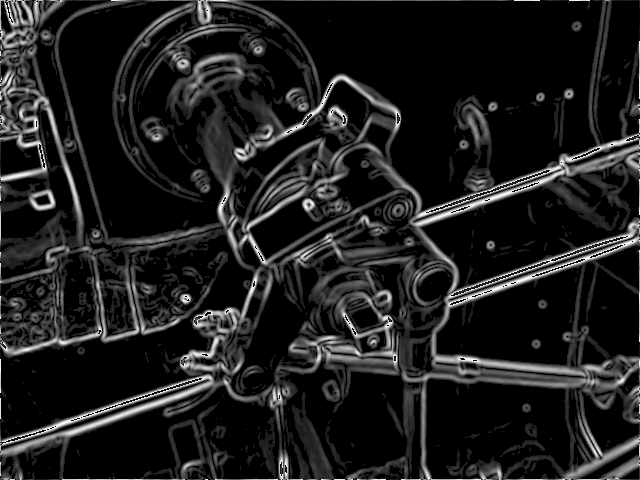
\includegraphics[width=1\linewidth,keepaspectratio]{../examples/valve/valve_gaussian-5x5_thresh-25}
				\subcaption{}
				\label{fig:sobelThreshCmp25}
			\end{subfigure} %
			\begin{subfigure}[b]{0.45\linewidth}
				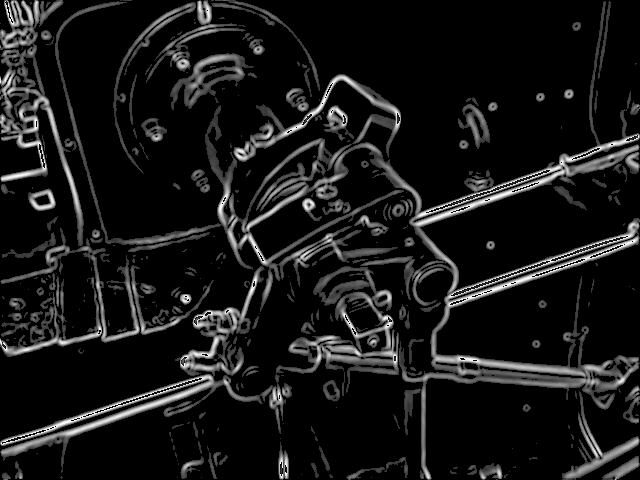
\includegraphics[width=1\linewidth,keepaspectratio]{../examples/valve/valve_gaussian-5x5_thresh-50}
				\subcaption{}
				\label{fig:sobelThreshCmp50}
			\end{subfigure} %
			\begin{subfigure}[b]{0.45\linewidth}
				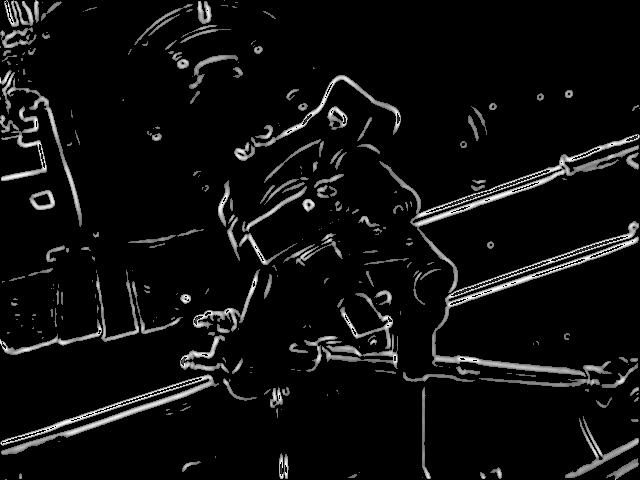
\includegraphics[width=1\linewidth,keepaspectratio]{../examples/valve/valve_gaussian-5x5_thresh-100}
				\subcaption{}
				\label{fig:sobelThreshCmp100}
			\end{subfigure} %
			\begin{subfigure}[b]{0.45\linewidth}
				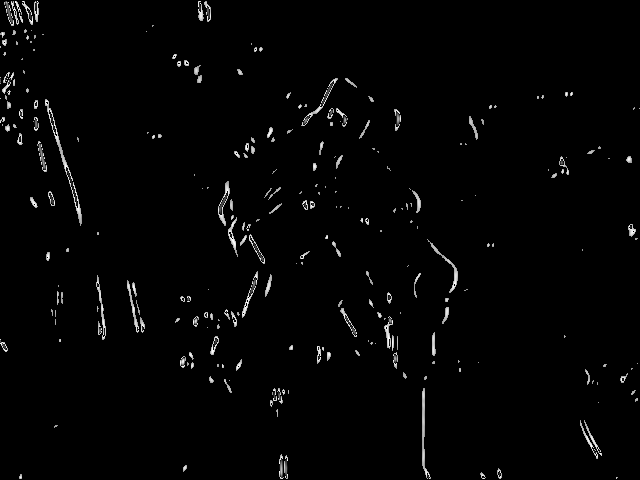
\includegraphics[width=1\linewidth,keepaspectratio]{../examples/valve/valve_gaussian-5x5_thresh-150}
				\subcaption{}
				\label{fig:sobelThreshCmp150}
			\end{subfigure} %
			\caption{\small Comparison of Sobel output for threshold values of (a) 25, (b) 50, (c) 100, and (d) 150. All were generated using a 5x5 Gaussian kernel with $\sigma = 3$.}
			\label{fig:sobelThreshCmp}
		\end{figure} %

		\autoref{fig:sobelThreshCmp} compares different threshold values of the Sobel algorithm for a Gaussian kernel of 5x5. The threshold values used are 25, 50, 100, and 150. This produces a much more drastic change than with the Gaussian kernel testing, though this is to be expected since the range of values here is only from 0 to 255. It has relatively the same affect as changing the kernel size in that increasing the threshold filters out fine details and leaves a sharper image with a fewer number of hard edges. This is the expected outcome as the threshold is designed to get rid of edges that have a lower intensity. From these two tests of the Sobel output, it can be concluded that the Sobel functionality was properly implemented. 

	\section{Conclusion}
		\label{sec:conclusion}
		In this project, a fully functional Sobel edge detector was created. The system takes in, through the testbench, the input file name and output file names so that it may read and write local files. Because of this, the implementation is not synthesizable. The project is able to grayscale the input image and then blur it using a reconfigurable Gaussian kernel that can be changed using a custom package written for this project. The source for this project has been posted online at \cite{github}.

		Now that the groundwork has been laid for image processing in VHDL, there are many potential future improvements for this system. Any other image processing technique or feature detector can be implemented using this as a backbone, as grayscaling and Gaussian blurring are the first steps to any feature detector. A notable next step for this project is to make it synthesizable. This should be an easy fix and would simply require streaming the file input data through the test bench into the source instead of using file I/O within the source files, as these are not synthesizable functions. The next closest improvement is Canny edge detection. This would simple require the implementation of one more component, saving a new two-dimensional array from the Sobel operator, calculating the gradient angles in addition to the magnitude, and using that to implement non-maximum suppression and hysteresis. 

	\begin{thebibliography}{00}
		\bibitem{canny} M. N. Teli, ``Canny edge detection,'' cs.umd.edu. [Online].Available: \url{https://www.cs.umd.edu/class/fall2019/cmsc426-0201/files/11_CannyEdgeDetection.pdf} (Accessed Apr. 30, 2020).

		\bibitem{canny2} P. K. Kalra, ``Canny edge detection,'' cse.iitd.ernet.in. [Online].Available: \url{www.cse.ittd.ernet.in/~pkalra/col783-2017/canny.pdf} (Accessed Apr. 30, 2020).

		\bibitem{io} E. Savas, ``VHDL basic i/o,'' sabanciuniv.edu. [Online].Available: \url{http://people.sabanciuniv.edu/erkays/el310/io_10.pdf} (Accessed Apr. 30, 2020).

		\bibitem{smoothing} R. Collins, ``Lecture 4: smoothing,'' cse.psu.edu. [Online].Available: \url{http://www.cse.psu.edu/~rtc12/CSE486/lecture04.pdf} (Accessed Apr. 30, 2020).

		\bibitem{book} R. Jain, R. Kasturi, and B. H. Schunck, ``Edge detection,'' in \textit{Machine Vision}, McGraw-Hill, 1995, ch. 5, pp. 140-185. [Online].Available: \url{https://www.cse.usf.edu/~r1k/MachineVisionBook/MachineVision.files/MachineVision_Chapter5.pdf} (Accessed Apr. 30, 2020).

		\bibitem{files} J. N. Moorkanikara, ``File declaration,'' ics.uci.edu. [Online].Available: \url{https://www.ics.uci.edu/~jmoorkan/vhdlref/filedec.html} (Accessed Apr. 30, 2020).

		\bibitem{github} [Online].Available: \url{https://github.com/NickChiapputo/VHDL_FeatureDetection}
	\end{thebibliography}
\end{document}